\textcolor{blue}{Problem 2}

9.2 Two-look Gaussian channel

\begin{figure}[htbp]
    \centering
	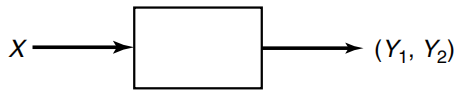
\includegraphics[width=0.4\textwidth]{../figure/9_1_9_2.png}
\end{figure}
Consider the ordinary Gaussian channel with two correlated looks at $X$, that is, $Y=\left(Y_1, Y_2\right)$, where
\begin{align*}
& Y_1=X+Z_1 \\
& Y_2=X+Z_2
\end{align*}

with a power constraint $P$ on $X$, and $\left(Z_1, Z_2\right) \sim \mathcal{N}_2(0, K)$, where

$$
K=\left[\begin{array}{ll}
N & N\rho \\
N\rho & N
\end{array}\right]
$$

Find the capacity $C$ for

(a) $\rho=1$

(b) $\rho=0$

(c) $\rho=-1$

\textcolor{blue}{Solution}
$$C=\max\limits_{p(x)}\ I(X;Y_1,Y_2)$$
\begin{align*}
I(X;Y_1,Y_2) &= h(Y_1,Y_2) - h(Y_1,Y_2|X) \\
&= h(Y_1,Y_2) - h(Z_1,Z_2|X) \qquad \left(\text{since } Y_i=X+Z_i\right) \\
&= h(Y_1,Y_2) - h(Z_1,Z_2) \qquad\quad\ \left(\text{since } Z_i\perp X\right)
\end{align*}
Since $\left(Z_1,Z_2\right)\sim\mathcal{N}_2(0,K)$, and $|K|=N^2(1-\rho^2)$, we have
$$h(Z_1,Z_2)=\frac{1}{2}\log\left((2\pi e)^2|K|\right)=\frac{1}{2}\log\left((2\pi e)^2 N^2(1-\rho^2)\right)$$
And since $Y_i=X+Z_i$, and since $X\perp Z_i$, so
\begin{align*}
\Var(Y_i) &= \Var(X+Z_i)=\Var(X)+\Var(Z_i)=\Var(X)+N \\
\Cov(Y_1,Y_2) &= \Cov(X+Z_1,X+Z_2)=\Var(X)+\rho N
\end{align*}
So the covariance matrix of $\left(Y_1,Y_2\right)$ is
$$K_Y=\left[\begin{array}{ll}
\Var(Y_1) & \Cov(Y_1,Y_2) \\
\Cov(Y_1,Y_2) & \Var(Y_2)
\end{array}\right]=\left[\begin{array}{ll}
\Var(X)+N & \Var(X)+\rho N \\
\Var(X)+\rho N & \Var(X)+N
\end{array}\right]$$
$$\Rightarrow |K_Y|=2\Var(X)N(1-\rho)+N^2(1-\rho^2)$$
Since $\rho\in[-1,1]\Rightarrow 1-\rho\geq 0$, and since $\Var(X)\leq P$, so we can get that
$$|K_Y|_{\max}=2PN(1-\rho)+N^2(1-\rho^2)$$
So
$$h(Y_1,Y_2)\leq\dfrac{1}{2}\log\left[(2\pi e)^2|K_Y|_{\max}\right]=\dfrac{1}{2}\log\left[(2\pi e)^2\left(2PN(1-\rho)+N^2(1-\rho^2)\right)\right]$$
So
\begin{align*}
C &= \max_{p(x),\Var(X)\leq P} I(X;Y_1,Y_2) \\
&= \dfrac{1}{2}\log\left(\dfrac{2PN(1-\rho)+N^2(1-\rho^2)}{N^2(1-\rho^2)}\right) \\
&= \dfrac{1}{2}\log\left(1+\dfrac{2P}{N(1+\rho)}\right)
\end{align*}

If and only if $X\sim\mathcal{N}(0,P)$, and $(Y_1,Y_2)\sim\mathcal{N}_2\left(\mathbf{0},\left[\begin{array}{ll}
P+N & P+\rho N \\
P+\rho N & P+N
\end{array}\right]\right)$,then $C$ takes the maximum value among $I(X;Y_1,Y_2)$.

(a) $\rho=1:$ \\
$$C = \dfrac{1}{2}\log\left(1+\dfrac{P}{N}\right) \text{ bits per transmission}$$

(b) $\rho=0:$ \\
$$C = \dfrac{1}{2}\log\left(1+\dfrac{P}{2N}\right) \text{ bits per transmission}$$

(c) $\rho=-1:$ \\
$$C = +\infty \text{ bits per transmission}$$

\newpage